%%%%%%%%%%%%%%%%%%%%%%%%%%%%%%%%%%%%%%%%%
%% Empirical section
\section{Empirical Framework}
\label{sec:empirics}

A professor is employed by a university, so it stands to reason that when public universities experience a secular fall in one of their revenue sources revenue --- analogous to a demand shock in the private sector --- that the composition of their employees will be affected.

Na\"ively we can analyse the relationship between professor-outcomes $Y_{i,t}$ at university $i$ in year $t$ as a result of state funding per student $X_{i,t}$.
Outcomes include count of professors per student within each university-year.
This model gives $\beta$ the association with these outcomes and state funding per student,\footnote{
    Note that dividing by student count also implicitly controls for the size of the university, so that this model accounts for yearly variation in professor count and university revenues arising from growth in a university.
}
including fixed effects to control for effects specific to the university and year.
Log$(.)$ transforming the variables improves the interpretability of $\beta$ as an elasticity for professor count per student with respect to state funding per student.
\begin{equation}
    \label{eqn:naivereg}
    Y_{i,t} = \alpha_i + \gamma_t + \beta X_{i,t} + \epsilon_{i,t}
\end{equation}

Yet a university's finances are not exogenous to state decisions for support of higher education, or exogenous to internal institutional decisions.
Instead, the state government and university administration undertake a complex process of allotting resources across multiple different priorities, including instruction, research, or between departments.
Importantly for this analysis, revenues received from an institution's state government provide opportunity to address this endogeneity.


\subsection{State Appropriation Shocks}
\label{sec:approp-shocks}

\cite{NBERw23736,chakrabarti2018effect,NBERw27885} address endogeneity in public university finances by exploiting a shift-share instrument for changes in state-level funding interacted with university reliance on state funding in a base period.
\begin{align}
    \label{eqn:public-instrument}
    Z_{i,t} &\coloneqq - \log \left[
    \left( \frac{\text{Total State Funding}_{s(i),t}}{\text{Student Population}_{s(i),t}} \right)
    \sum_{\tau = 0}^{3} \frac 14
    \left( \frac{\text{State Funding}_{i,1990 + \tau}}{\text{Total Revenues}_{i,1990 + \tau}} \right) \right]
\end{align}
The system exploits the fact that institutions who rely on state appropriations more will be affected by state appropriation shocks.
$Z_{i,t}$ is the instrument for (log) state appropriations for institution $i$ in year $t$, interacting the average funding for universities in state $s(i)$ with reliance on state funding relative to total revenues, averaged across the base years 1990--1993.\footnote{
    1990--1993 are defined as data for public university finance data are most comparable (i.e. without many missing values) beginning in 1990.
    \cite{NBERw23736} use the single year 1990 as the base year, though I use the four years to ameliorate missing values in the single year of 1990.
    Results are similar in either specification.
}
$Z_{i,t}$ is contructed as negative to reflect the fact that the long term trend in, and most of the short-run shocks to, state funding for higher education has been negative.
State funding has been been falling, so that the instrument describes shocks to university revenues, mostly in a negative direction.

\cite{NBERw27885} notes the tendency for public universities to respond to state funding cuts by increasing reliance on tuition, where \cite{NBERw23736} specifically instruments for tuition revenues with collected information on legislative tuition price controls.\footnote{
    \label{foot:control}
    It may be argued that tuition revenues are confounder between the causal effect of changes in state funding on a university's total revenues, so that this analysis focuses on state support for higher education (no total revenue) as a result.
    This follows the \cite{NBERw27885} formulation.
    On the other hand, rises in tuition revenues (per student) may arise as result of tuition hikes thanks declining state support, which would mean controlling for tuition would constitute a bad control.
    Estimates including tuition revenues (per student) as a control in the second stage of the IV estimates produces results of very similar magnitude and direction, and so are omitted.
}
This analysis focuses on one important source of revenues for public universities: state appropriations.

The first-stage is then as follows, including institution and year fixed effects.
\begin{equation}
    \label{eqn:firststage}
    X_{i,t} = \eta_i + \zeta_t + \delta Z_{i,t} + \epsilon_{i,t}
\end{equation}
We note the conditions for exogeneity in the instrument (following the discussion presented by \citealt{NBERw27885}).
The instrument is exogenous if state policy decisions for funding of public universities are uncorrelated with unobserved institutional changes of any specific college or university in the state \citep{borusyak2022quasi}.
This assumption is plausible given that the majority of states have multiple (i.e. more than five) public universities, without any single university campus receiving the majority of state funding within any single state.
Secondly, addressing endogeneity in university revenues by the shift-share identification strategy requires exogeneity in either the base-line share or shift component of the instrument.
In this case, we satisfy the second: universities' institutional-level decisions are not correlated with contemporaneous or upcoming shocks to state appropriations.\footnote{
    It would be plausible to consider the case that universities make institutional-level decisions in a consistently different manner to those 
    with differing reliance on state appropriations in 1990, so that exogeneity by the base-line share is not plausible here.
}

\begin{table}[h!]
    \singlespacing
    \centering
    \caption{First Stage Estimates, for State Funding by Appropriation Shock.}
    \makebox[\textwidth][c]{
\begin{tabular}{@{\extracolsep{5pt}}lcccc} 
\\[-1.8ex]\hline 
\hline \\[-1.8ex] 
 & \multicolumn{4}{c}{Dependent Variable: Non-institutional Revenues} \\ 
\cline{2-5} 
\\[-1.8ex] & (1) & (2) & (3) & (4)\\ 
\hline \\[-1.8ex] 
 Appropriations Shock & 0.990 & 0.608 & 0.980 & 0.350 \\ 
  & (0.075) & (0.059) & (0.078) & (0.084) \\ 
  Tuition Revenue & 0.063 & 0.558 &  &  \\ 
  & (0.055) & (0.059) &  &  \\ 
  Constant &  & $-$0.982 &  & 6.011 \\ 
  &  & (0.751) &  & (0.688) \\ 
 \hline \\[-1.8ex] 
Uni. + Year fixed effects? & Yes & No & Yes & No \\ 
F stat. & 92.461 & 88.72 & 156.791 & 17.487 \\ 
Observations & 18,504 & 18,504 & 18,504 & 18,504 \\ 
R$^{2}$ & 0.801 & 0.222 & 0.801 & 0.064 \\ 
\hline 
\hline \\[-1.8ex] 
\end{tabular} 
}
    \label{tab:firststage-reg}
    \begin{flushleft}
        \footnotesize
        \textbf{Note}: Standard errors are clustered at the state-year level.
    \end{flushleft}
\end{table}

\autoref{tab:firststage-reg} presents results of the first-stage regression, separately with and without a control for tuition revenue per student, plus institution and year fixed effects.\footnote{
    Representations for frequentist significance levels (i.e. 10, 5, 1\% etc.) are omitted here, and in all following tables.
}
We note columns (1) and (2) estimate that a shock to appropriations (per student in the entire state) of 10\% is associated with 9.8\% change in state funding per student at the university; the instrument is strong, and we note similarity in estimates with and without inclusion of fixed effects.
Columns (3) and (4) include the tuition revenue control (explained in \autoref{foot:control}) to exhibit estimates with the inclusion of this possible collider or bad control.
Column (3) shows similar estimates to columns (1), (2) thanks to inclusion of fixed effects, so that the fixed effects was effective in soaking variation in per-student tuition revenues at the institution-year level.
Column (1) represents the estimates for \autoref{eqn:firststage} with fixed effects, omitting the tuition revenue control, and is the preferred form that I proceed with in the following.

\begin{figure}[h!]
    \centering
    \singlespacing
    \caption{Local Projection Estimates for First-Stage \autoref{eqn:firststage}.}
    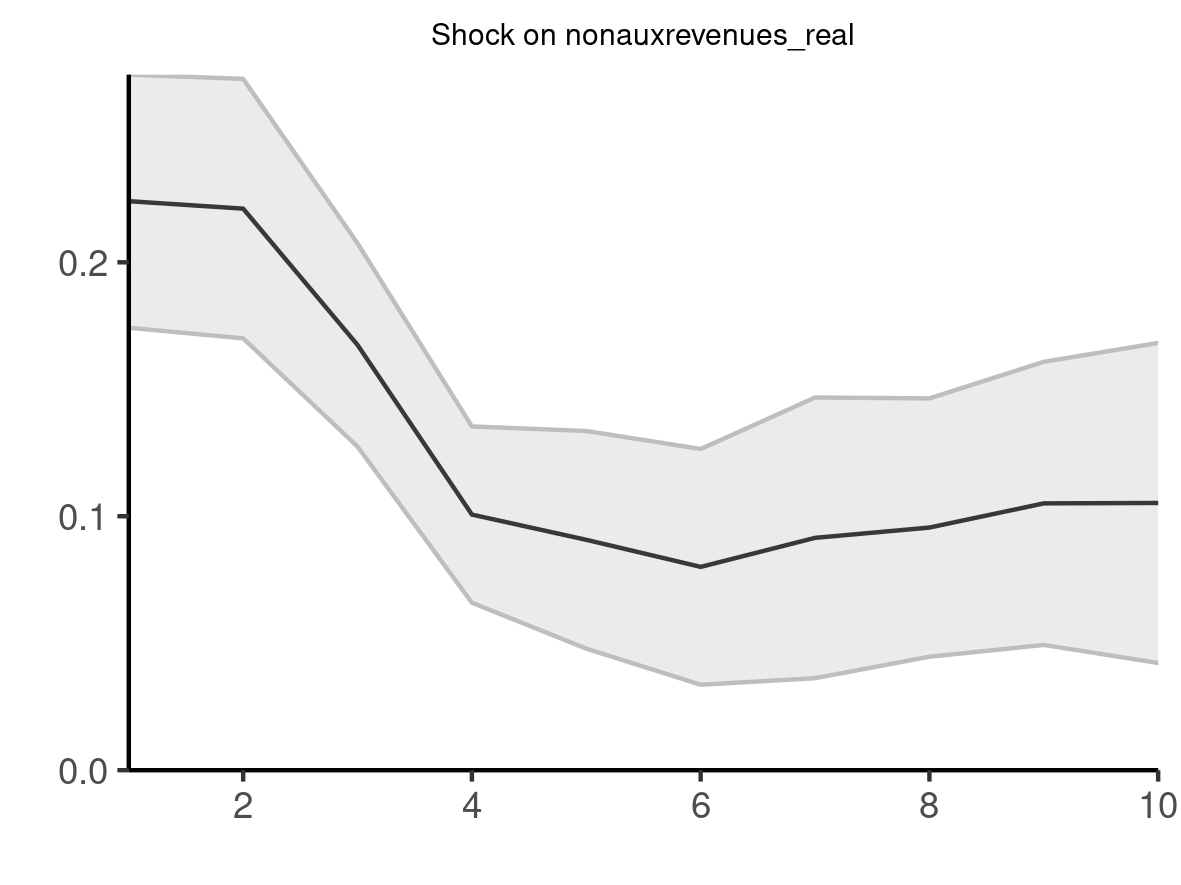
\includegraphics[width=0.6\textwidth]{figures/firststage-lp.png}
    \label{fig:firststage-lp}
\end{figure}

\autoref{fig:firststage-lp} presents local projection estimates for the staying-power of the state appropriation shock to university revenues, with each year showing the years following effect of a shock to state reveunes in year zero.
We see a decaying, yet real and positive, effect of the shock on revenues for the next 10 years, illustrating that the state appropriation shock is a strong, if fading, instrument for state funding per student and justifying its use in local projection IV estimation.

These results, together with the case for exogeneity, show the appropriations shock instrument strongly predicts university revenues in the first-stage estimation.


\subsection{Instrumental Variables Model, University-Level}
\label{sec:iv-model-uni}

The primary empirical model combines the instrumental variable for state appropriation shocks with the empirical model for the effects of state funding at the university-level --- i.e. parameter $\beta$ in the following.\footnote{
    It is important to note the treatment effect isolated here; the instrumental variables approach identifies the local average treatment effects (LATE) specific to the instrument.
    So we interpret this treatment effect as a university's response in employment count and average salaries to state funding changes, changes specific to state appropriation shocks, among the complier group --- i.e. universities with any exposure to shocks, assuming no universities increase employment or salaries in response to negative revenue shocks.
    \cite{mogstad2021causal} provide a full discussion of the LATE with instruments and multiple monotonicity conditions.
}
\begin{eqnarray}
    \label{eqn:secondstage1}
    X_{i,t} &=& \eta_i + \zeta_t + \delta Z_{i,t} + \epsilon_{i,t} \\
    \label{eqn:secondstage2}
    Y_{i,t} &=& \alpha_i + \gamma_t + \beta \widehat X_{i,t} + \varepsilon_{i,t}
\end{eqnarray}
I estimate the system by two stage least squares, including institution and year fixed effects, and investigate outcomes at the university-level to analyse effects on the university as a result of changes in revenues.
Additionally, I estimate the model via local projections \citep{jorda2005,miller2022} to investigate whether the effects of revenues on faculty composition linger for multiple years after the original appropriation shock.
Regarding outcomes, I focus on the composition of the professors employed at the university by analysing (log) count per student, and average salaries paid to, professors employed by the university.

\begin{figure}[H]
    \centering
    \singlespacing
    \caption{Instrument Variables Model for University Finances and Faculty Composition.}
    \begin{tikzpicture}
        \node[state] (instrument) at (0,0) {$Z$};
        \node at (-2.6,0.5){State};
        \node at (-1.9,0){appropriation};
        \node at (-2.6,-0.5){shock};
        \node[state] (endogenous) [right=of instrument] {$X$};
        \node at (2,1.5) {University};
        \node at (2,1) {revenues};
        \node[state] (outcome) [right=of endogenous] {$Y$};
        \node at (5.2,0.25) {Faculty};
        \node at (5.6,-0.25) {Composition};
        % Relevance condition
        \path (instrument) edge (endogenous);
        \path (endogenous) edge (outcome);
        % Exclusion Restriction
        \path (instrument) edge[bend right=60] (outcome);
        \node[color=red] at (2,-1.2) {X};
    \end{tikzpicture}
    \label{fig:SCM-ivmodel}
\end{figure}

\autoref{fig:SCM-ivmodel} presents the system in graphical form, for the causal effect of state appropriation shocks on university revenues and thus faculty composition, making clear the assumption that appropriation shocks affect faculty composition only via affecting university finances.


\subsection{Instrumental Variables Model, Individual Professor-Level}
\label{sec:iv-model-indiv}

This analysis additionally uses data regarding individual professors in the Illinois university system, to investigate the effects of changes in university revenues on the individual professors at the universities.
Redefining the level of outcome requires adjustment to the empirical approach, leveraging variation in university finances for the years after a professor joins the university.\footnote{
    This formulation follows that presented by \cite{NBERw27885}, where individual student outcomes are analysed via variation in state appropriations after their freshman-year.
    This contrasts with \autoref{sec:iv-model-uni} and \cite{NBERw23736}, where the unit of analysis is the university-year.
}

\autoref{eqn:rolling-instrument} defines a rolling-share variant of the instrument, $\tilde Z_{j,t}$, where the university's state appropriations share exposure is based in the year a professor joins the university --- and not the base period 1990--1993.
$j$ indexes each professor in year $t$, $\tau(j)$ for the year the professor first joins their institution.\footnote{
    Identifying $\tau(j)$ is possible for $j$ by restricting to all professors hired 2011-2021 --- i.e. in the years after the start of the full panel.
    It is not possible to discern the hiring year for professors who  were hired in the years preceding 2011, and so the entire sample is only possible to analyse using the base-share in years 1990-1993 formulation (e.g., \autoref{tab:facultysalaries-shock-illinois}, \ref{tab:promotion-shock-illinois}).
}
\begin{align}
    \label{eqn:rolling-instrument}
    \tilde Z_{j,t} &\coloneqq - \log \left[
    \left( \frac{\text{Total State Funding}_{s(j),t}}{\text{Student Population}_{s(j),t}} \right)
    \left( \frac{\text{State Funding}_{\tau(j)}}{\text{Total Revenues}_{i,\tau(j)}} \right) \right]
\end{align}

This approach leverages an insight, made available by level of the data: that an individual professor is affected by changes in university revenues after they have joined the university.\footnote{
    Notice that \autoref{sec:iv-model-uni} considers the number of professors employed by the university; whether a professor becomes employed at the university is likely affected by that university's finances.
    The formulation in this section does not consider whether the professor joins the university, instead taking as given that the professor is employed at the university, and then projects the effect on the individual.
}
Exogeneity and relevance of the rolling-share instrument, $\tilde Z_{j,t}$, follows the same reasoning as that for the base-share instrument, $Z_{i,t}$, discussed in \autoref{sec:approp-shocks}.\footnote{
    The base-share instrument is appropriate for some outcomes with the individual Illinois professors, where appropriate (\autoref{tab:facultysalaries-shock-illinois}, \ref{tab:promotion-shock-illinois}).
}
We satisfy the assumptions for exogeneity by noting that none of the Illinois public campuses take the majority of state appropriations, and that the instrument identification strategy relies on exogeneity in changes in state appropriations to individual professor-outcomes, following the year they joined the university.\footnote{
    Additionally, within-institution changes resulting from share reliance on state funding may be correlated with unobserved changes in the outcomes, so that \cite{NBERw27885} note the importance of controlling for the base share and state student population.
    The formulation here implicitly controls for these factors via the fixed effects; results are relatively similar while including these controls without including fixed effects, and so are omitted.
}
\autoref{tab:firststage-illinois} presents results of the first stage estimation, showing that the instrument is strong in the same way as that for the university-level outcomes (\autoref{tab:firststage-reg}), with very similar estimates for the association between appropriation shocks and non-institutional revenues.

The instrumental variables model is then defined as follows where $i(j)$ refers to the institution that professor $j$ is employed at, and $Y_{j,t}$ refers to individual-level outcomes total salary, rate of promotion, and propensity to leave the Illinois public university system.
The system includes a fixed effect for the institution and first year of employment.\footnote{
    The instrument varies by institution, based in the year of first employment, so that these are the corresponding fixed effects and levels of clustered standard errors.
}
\begin{eqnarray}
    \label{eqn:secondstage1_indiv}
    X_{i(j),t} &=& \theta_{i(j)} + \phi_{\tau(j)} + \delta \tilde Z_{i(j),t} + \epsilon_{i(j),t} \\
    \label{eqn:secondstage2_indiv}
    Y_{j,t} &=& \mu_{i(j)} + \nu_{\tau(j)} + \beta \widehat X_{i(j),t} + \varepsilon_{j,t}
\end{eqnarray}
We then interpret parameter $\beta$ as the effect of changes in state funding at an Illinois public university, via state appropriation shocks, on an individual professor's outcome $Y_{j,t}$.
